\documentclass[12pt,a4paper]{article}
\pagestyle{plain}
\usepackage{fullpage}
\usepackage[english]{babel}
\usepackage{enumerate}


%equations
\usepackage[fleqn]{amsmath}
\numberwithin{equation}{section}

%figures
\usepackage[dvips]{graphicx}
\graphicspath{{./images/}}
\numberwithin{figure}{section}

%excercises
\newcounter{Exercise}
\setcounter{Exercise}{1}
\usepackage[dvipsnames]{xcolor}
\usepackage{framed}
\definecolor{shadecolor}{gray}{0.9}
\usepackage{caption}

%tables
\numberwithin{table}{section}

%specials
\usepackage{textcomp} %special (greek) characters as text
%\usepackage{pstricks} %
%\usepackage{ifthen} %
%\usepackage{calc} %
%\usepackage{isotope}
\usepackage{hyperref}
\usepackage[bottom]{footmisc} %footnote below figure
\usepackage{footnpag}%number footnotes per page
\usepackage{nicefrac}%fractions with slash


%document details
\author{N.G. Schultheiss \\ translated and adapted by K. Schadenberg}
\date{}
\title{Standard Model - Particles}


\begin{document}
\maketitle

\section{Introduction}
A powerful tool (model) particle physicists have at their disposal when trying to make sense of the world around us is the Standard Model. In this module and the next (`Standard Model - Forces') we will take a closer look at this model: How did it develop and what particles does it describe.

\section{Early Particle Physics}
Around the year 1900 there was a lot of research going on focussed on discovering the structure and composition of atoms. Joseph John Thomson (1856-1940) imagined atoms as `plum puddings'; negative electrons (which he discovered) distributed and moving rapidly in a sea of positive charge. This model however was not correct as Johannes Wilhelm Geiger\footnote{Best known as the co-inventor of the Geiger-M\"uller counter together with Walther M\"uller (1905-1979).} and Ernest Marsden (1889-1970), two students of Ernest Rutherford (1871-1937), showed with an experiment in 1909. They irradiated a gold foil with radiation coming from Radium. Most of the radiation passed unhindered through the foil, only a small part was reflected or refracted. Their explanation: an atom consist of a small hard kernel (the nucleus) surrounded by a cloud of electrons.

\begin{figure}\begin{center}
\begin{picture}(0,0)%
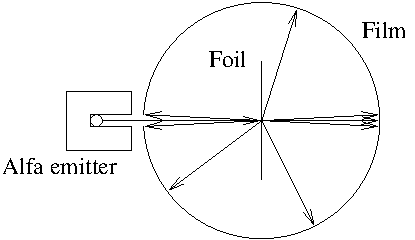
\includegraphics{rutherford}%
\end{picture}%
\setlength{\unitlength}{4144sp}%
%
\begingroup\makeatletter\ifx\SetFigFont\undefined%
\gdef\SetFigFont#1#2#3#4#5{%
  \reset@font\fontsize{#1}{#2pt}%
  \fontfamily{#3}\fontseries{#4}\fontshape{#5}%
  \selectfont}%
\fi\endgroup%
\begin{picture}(3159,1818)(-869,-970)
\end{picture}%
\caption{The Rutherford experiment.}\label{fig:rutherford}
\end{center}\end{figure}

The next step in research was to find out if that tiny kernel had any structure. Around 1919 Rutherford came to the conclusion that atomic nuclei can be transformed by irradiating them with $\alpha$-particles (Helium nuclei). These particles were able to change the positive charge of the nucleus. But the chemical properties of the nuclei also changed. This observation led to the discovery of the proton. The model was made complete by James Chadwick (1891-1974) in 1932 with the discovery of the neutron.

The three different particles, electrons, protons, and neutrons, can be distinguished by two characteristic properties; mass and charge. Together they can form atoms. Some of these atoms are stable, but other are not and decay. We call these atoms radioactive because they emit radiation during their decay. A characteristic property of a radioactive element is its half-life (or decay constant), when a time period of one half-life has expired in intensity of radiation had decreased by 50\%.

In 1922 Otto Stern (1888-1968) and Walther Gerlach (1889-1979) showed that silver atoms (as a whole) have a `spin'. The silver atoms were shot through an inhomogeneous magnetic field at a large screen. This screen showed two spots of silver atoms and not the expected continuous line. The only possible conclusion was that the silver atoms can only have certain fixed (quantised) magnetic properties; spin.\footnote{Apparently there is such a thing as an elementary magnet, just like the elementary charge.} A few years later in 1926, Samuel Abraham Goudsmit (1902-1978) and George Eugene Uhlenbeck (1900-1988) showed that individual electrons also have a spin.

The composition of atoms was now known, but the exact structure was still a bit unclear. Is there is certain order or structure in the clouds of electrons around nuclei? This was the field of research of Niels Bohr (1885-1962), Erwin Schr\"odinger (1887-1961) and many others. The electrons are not randomly distributed in the cloud, instead they have certain orbits. But the calculations involving these orbits let to a new kind of physics, quantum mechanics. The module `de Broglie' shows the orbits for the simplest atom we know, the hydrogen atom. An electron inside the hydrogen atom cannot have any arbitrary energy, because the orbits are fixed the energies are also fixed. This in turn leads to fixed energy steps between orbits. These fixed energy transitions are the explanation behind absorption and emission lines (see modules `Colour' and `Fluorescence').

Electrons are charged particles, this means that they can be manipulated by magnetic fields. The spin of an electron can be aligned parallel or anti-parallel (pointing in the opposite direction) to an external field. The two orientations have different energies. Zeeman showed that every line in an emission spectrum can be split into two using magnetic fields. The difference in magnetic energy is the basis for a medical imaging technique called Magnetic Resonance Imaging (MRI).

\section{Particle Accelerators}
During World War II a lot of research in the field of particle physics was aimed at developing atomic weapons. This research continued after the war. But there was always room for more fundamental research. After the war newly developed particle accelerators where used to probe into the insides of atoms. Accelerators can be broadly classified into two categories: linear accelerators and cyclotrons or circular accelerators.

\subsection{Linear Accelerators}
In 1945 Luis Walter Alvarex (1911-1988) used materials left over after the war to build a linear accelerator. A linear accelerator is a long vacuum tube in which charged particles are accelerated using electrical fields. Inside the tube there are conducting rings connected to an alternating current power supply. Equal charges repel while opposite charges attract, this allows one to accelerate the charged particles. The particle in figure~\ref{fig:lineac} is repelled by the first ring on the left hand side of the tube and is attracted by the second ring. When the particle passes through the second ring the power supply changes the polarity of the rings. Now the second ring repels the particle while the third ring attracts. This series of rings transforms electrical energy ($E=q \cdot \Delta V$) into kinetic energy ($E= \frac{1}{2}mv^2$). Calculating the energy of the particle (in eV) at the end of the tube is now a simple matter of multiplying the charge of the particle with the voltage between two consecutive rings.

\begin{figure}\begin{center}
\begin{picture}(0,0)%
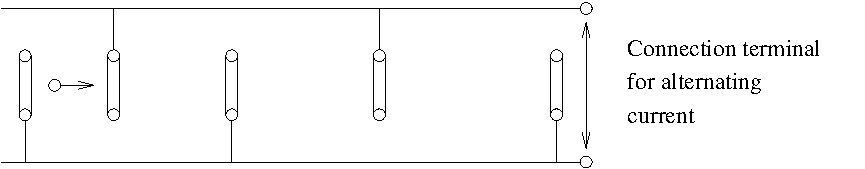
\includegraphics{lineac}%
\end{picture}%
\setlength{\unitlength}{4144sp}%
%
\begingroup\makeatletter\ifx\SetFigFont\undefined%
\gdef\SetFigFont#1#2#3#4#5{%
  \reset@font\fontsize{#1}{#2pt}%
  \fontfamily{#3}\fontseries{#4}\fontshape{#5}%
  \selectfont}%
\fi\endgroup%
\begin{picture}(6581,1276)(259,-474)
\end{picture}%
\caption{Schematic representation of a linear accelerator.}\label{fig:lineac}
\end{center}\end{figure}

\begin{shaded}
\textbf{Exercise \theExercise \stepcounter{Exercise}} : Convert 6.6~GeV into Joules.\end{shaded}
\begin{shaded}
\textbf{Exercise \theExercise \stepcounter{Exercise}} : Calculate the speed of a proton after it passed through five rings of a linear accelerator. Assume that the proton was stationary at the first ring. The voltage between the rings is 1~kV.\end{shaded}
\begin{shaded}
\textbf{Exercise \theExercise \stepcounter{Exercise}} : Explain why the distance between the rings in figure~\ref{fig:lineac} increases over the length of the tube.\end{shaded}

\subsection{Cyclotrons}
The number of rings inside a linear accelerator limits the amount of energy which can be pumped into the particles. A cyclotron does not have this limitation because the particles circle or spiral around inside the accelerator. With every rotation inside the accelerator the particle can get a little bit more energy. A magnetic field is used to keep the particles in a circular orbit.

\begin{figure}\begin{center}
\begin{picture}(0,0)%
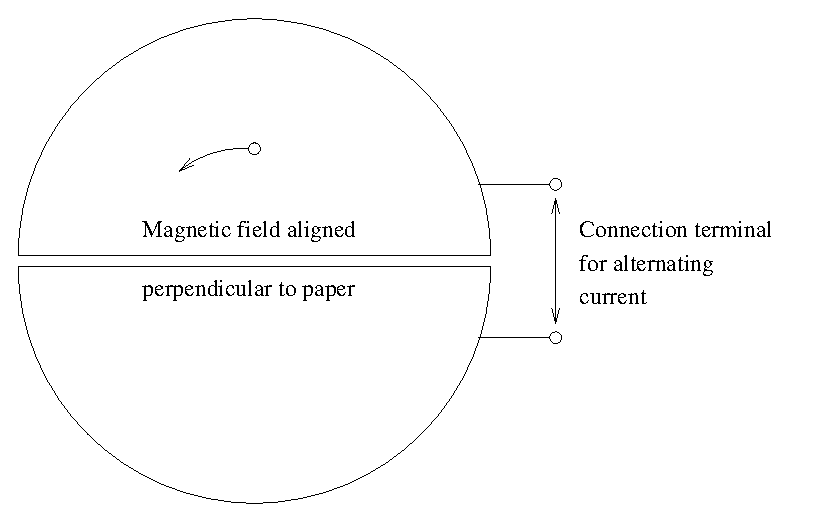
\includegraphics{cyclotron}%
\end{picture}%
\setlength{\unitlength}{4144sp}%
%
\begingroup\makeatletter\ifx\SetFigFont\undefined%
\gdef\SetFigFont#1#2#3#4#5{%
  \reset@font\fontsize{#1}{#2pt}%
  \fontfamily{#3}\fontseries{#4}\fontshape{#5}%
  \selectfont}%
\fi\endgroup%
\begin{picture}(6086,3708)(79,-4030)
\end{picture}%
\caption{Schematic representation of a cyclotron.}\label{fig:cyclotron}
\end{center}\end{figure}

Every time a particle in figure~\ref{fig:cyclotron} completes one half of an orbit it gets a boost from the electrical field. Because the speed of the particle increases, but the magnetic field stays the same, the orbit of the particle will get larger (larger radius). This is not the only limitation to the acceleration. Nothing can go faster than light (in vacuum) according to Einstein. When the particle approaches this speed a part of the extra energy obtained from the electrical field is converted into mass\footnote{$E=mc^2$!} instead of velocity.

\begin{shaded}
\textbf{Exercise \theExercise \stepcounter{Exercise}} : Suppose the cyclotron is fed with an alternating current of a fixed frequency. What can you say about the orbital period of the particle inside the cyclotron? How can this particle then still increase its velocity?\end{shaded}

Ernest Orlando Lawrence (1901-1958) started developing cyclotrons in 1929. Years of research led to the development and building of the Bevatron (\textbf{B}illions of \textbf{eV} Synchro\textbf{tron}) at the Lawrence Berkeley National Laboratory in 1954. With this accelerator protons were accelerated up to energies of 6,6~GeV. According to Einstein, at this energy the protons have a mass of $6.6~\frac{\mbox{GeV}}{c^2}$.

\begin{shaded}
\textbf{Exercise \theExercise \stepcounter{Exercise}} : Calculate the increase in mass of the protons, as a multiple of the original (rest) mass of a proton, when they have an energy of 6.6~GeV.\end{shaded}

1~GeV is $1 \cdot 10^9$~ eV or one billion electron Volts. Before 1974 the United Kingdom used the long scale to name large numbers. In the long scale a billion is $1 \cdot 10^{12}$. Luckily, in 1954 de United States, where the Bevatron was build, already used the short scale, making the naming of the machine now correct on both sides of the Atlantic.\footnote{Except that the rest of Europe still uses the long scale \ldots}

The Bevatron was designed in order to verify the hypotheses that every particle had a corresponding anti-particle of opposite charge but identical in all other aspects.\footnote{Better known as charge symmetry.}  The anti-electron, or positron, was already discovered in cosmic rays in 1930. Shortly after the Second World War both positive and negative muons and pions were observed, also in cosmic ray experiments. What was missing was the anti-proton. In order to create such a particle, physicists calculated that the proton beam from the Bevatron, which was aimed at a fixed target, should have an energy of at least 6.2~GeV. Not only did the Bevatron confirm the existence of anti-protons in 1955, but one year later the anti-neutron was also discovered.

Our list of particles from the beginning of this module has now expanded quite a bit. We now have electrons and anti-electrons, protons and anti-protons, and neutrons and anti-neutrons. If we were to combine an anti-proton with an anti-electron we obtain an anti-hydrogen atom. This can happen during a number of different particle experiments, but the first to specifically make anti-hydrogen to study it was the LEAR (Low Energy Antiproton Ring) experiment at CERN in 1995.

The search for `new' particles did not stop after the discovery of the anti-proton and neutron. But ever larger and more powerful accelerators were needed. One could use cosmic rays to obtain high energy particles, in fact a lot of scientist did. But the drawback of cosmic rays is that one cannot control them. Were do you place your detector and what was the energy of you primary particle?

Not only were physicists looking for new particles, they were also trying to understand the known particles. Pions where thought to be a sort of glue holding the protons and neutrons together inside atoms. Were there also anti-pions and how does this glue work? For this the scientist also needed more powerful accelerators. To look inside the nucleus of an atom you need to be able to visualise very small structures and to do this you need particles with a very short wavelength i.e. a high energy (see the module `de Broglie').

The beam of protons inside the Bevatron had a cross section (aperture) of $\frac{1}{3}~\mbox{m}^2$. A large magnet was needed to keep the beam of protons spinning around. If the beam were smaller the magnet(s) could also be smaller and also allows us to create particles with higher energies. After Bevatron came Tevatron, this new accelerator was able to accelerate particles up 1~TeV, one tera electron volt. Tevatron was the most powerful accelerator in the world for a long time. But now this honour goes to the LHC (Large Hadron Collider) at CERN. The beams inside the LHC have a diameter of only 16~$\mu$m.

\begin{shaded}
\textbf{Exercise \theExercise \stepcounter{Exercise}} : Protons accelerated at the LHC circle around a 27~km long ring and are focussed inside a beam 16~$\mu$m thick. The moon is roughly 1~light second away from us. Calculate the thickness of the LHC bundle if the protons where orbiting at the same distance as the moon.  \end{shaded}

\section{Quarks}
Collision experiments have shown us that protons and neutrons consist of even smaller building blocks. The particles are called quarks, both the proton and neutron are built using three quarks.

We can draw a small scheme summarizing our knowledge up to now:
\begin{figure}[h]\begin{center}
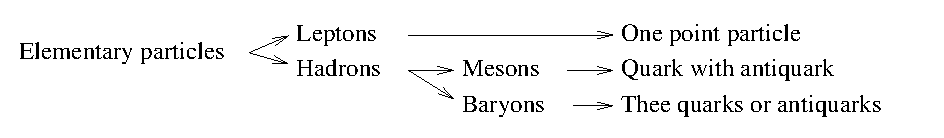
\includegraphics[scale=1]{particles.eps}
\label{fig:particles}
\end{center}\end{figure}

Leptons are particles like electrons, positrons, and neutrinos. Protons and neutrons consist of three quarks, they therefore must be baryons. Mesons will be discussed in further detail in the next module `Standard Model - Forces'.

A proton consists of two `up'-quarks and one `down'-quark. The neutron consists of two `down'-quarks and one `up'-quark. These quarks have anti-matter counter parts: anti-up and anti-down. These are needed to create anti-protons and anti-neutrons. These quarks were all found using the earliest particle accelerators, they are known as the first generation quarks. 

With bigger and more powerful accelerators heavier particles could be created. We now know there are at least three generations of quarks. Their names and a summary of their properties is given in table~\ref{tab:quarks}.

\begin{center}\begin{tabular}[h]{c c c r r} 
Generation & Name & Symbol & Spin & Q ($e$) \\ \hline
1 & Up & u & $\nicefrac{1}{2}$ & $\nicefrac{2}{3}$ \\
1 & Down & d & $-\nicefrac{1}{2}$ & $-\nicefrac{1}{3}$ \\
2 & Charm & c & $\nicefrac{1}{2}$ & $\nicefrac{2}{3}$ \\
2 & Strange & s & $-\nicefrac{1}{2}$ & $-\nicefrac{1}{3}$ \\
3 & Top & t & $\nicefrac{1}{2}$ & $\nicefrac{2}{3}$ \\
3 & Bottom & b & $-\nicefrac{1}{2}$ & $-\nicefrac{1}{3}$
\end{tabular}
\captionof{table}{Known quarks.}\label{tab:quarks}
\end{center}

This organisation of quarks is based on a model by Murray Gell-Mann (1929). He used group theory to develop his model known as SU(3) or Eightfold way. All quarks have a certain charge; quarks have a charge $\nicefrac{2}{3}~e$ or $-\nicefrac{1}{3}~e$ while anti-quarks have a charge $-\nicefrac{2}{3}~e$ or $\nicefrac{1}{3}~e$. But the (free) charges we find around us always have an integer number (-2, -1, 0, 1, etc.). Apparently there are certain rules for combining quarks to form larger particles.

\section{Fermions and Bosons}
An important property of particles is their spin (number). According to this number particles can be divided into two groups: Fermions and Bosons.
\subsection{Fermions}
Fermions are named after Enrico Fermi (1901-1954). They are particles with a half-integer spin i.e.:
\begin{equation}
n + \frac{1}{2}
\end{equation}
with $n$ an integer.

Every fermion must occupy a unique state. We will explain this statement using a simple atom as an example: the He-4 atom. The nucleus of this atom consists of two neutron and two protons. Around this nucleus orbit two electrons (giving the atom as a whole a neutral charge). If the atom is in its ground state (the lowest possible energy level) these electrons will occupy the electron shell (orbit) closest to the nucleus. At first glance it might seem as though these electrons are in the same state (energy level and position are the same). Their spin number however is different, one has spin $-\nicefrac{1}{2}$ the other $\nicefrac{1}{2}$. These are the only two spin number available to electrons, therefore a single electron shell cannot hold more than two electrons.

The fact two similar quantum states are forbidden is named after Wolfgang Ernst Pauli (1900-1958); the Pauli exclusion principle.

\subsection{Bosons}
Bosons are named after Satyendra Nath Bose (1894-1974). They are particles with a integer spin: $\ldots$, -2, -1, 0, 1, 2, $\ldots$.

The He-4 atom as a whole can be seen as a boson. It consists of six particles each with spin number $-\nicefrac{1}{2}$ or $\nicefrac{1}{2}$. Every possible (valid) combination of the building blocks of the He-4 atom will yield an integer spin.

The Pauli exclusion principle does not apply for bosons. Therefore a group of bosons can occupy the same quantum state. This can lead to some interesting phenomena. When He-4 is cooled to very low temperatures, near absolute zero, it forms a Bose-Einstein Condensate (BEC). The atoms start to behave as a single unit; a superfluid.

\begin{shaded}
\textbf{Exercise \theExercise \stepcounter{Exercise}} : Do a bit of online research to find out how a BEC behaves and what a superfluid is. You might find some interesting movie clips.\end{shaded}

\section{Leptons}
Leptons are a type of fermions which are, as far as we now know, indivisible. Leptons can therefore be seen as point particles. The most familiar lepton is the electron. In one of the earlier modules, `The Sun', we saw that the electron has an anti-particle counterpart: the positron. Both the electron and positron have heavier brothers: the muon and tauon. To make the family complete there are the slightly weird cousins: three types of neutrinos.

According to Einstein mass equals energy, the more massive you are the more energy you have. Particles can lose some of their energy. They decay into lighter particles.

The table below summarises a part of our knowledge of the lepton family.

\begin{center}\begin{small}
\begin{tabular}[h]{l c r r r r r r r r} 
Name & Symbol & Spin & Q ($e$) & L$_e$ & L$_{\mu}$  & L$_{\tau}$  & Mass ($\frac{\mbox{MeV}}{c^2}$) & half-life (s) \\ \hline \hline
Electron & $e^+$ & -1 & $\nicefrac{1}{2}$ & +1 & 0 & 0 & 0.510998910 & Stable \\ 
Positron & $e^-$ & +1 & $\nicefrac{1}{2}$ & -1 & 0 & 0 & 0.510998910 & Stable \\ \hline
Muon & $\mu^+$ & -1 & $\nicefrac{1}{2}$ & 0 & +1 & 0 & 105.6583668 &  $2.197 \cdot 10^{-6}$ \\ 
Anti-muon & $\mu^-$ & +1 & $\nicefrac{1}{2}$ & 0 & -1 & 0 & 105.6583668 & $2.197 \cdot 10^{-6}$ \\ \hline
Tauon & $\tau^+$ & -1 & $\nicefrac{1}{2}$ & 0 & 0 & +1 & 1,776.84 & $2.906 \cdot 10^{-13}$ \\ 
Anti-tauon & $\tau^-$ & +1 & $\nicefrac{1}{2}$ & 0 & 0 & -1 & 1,776.84 &  $2.906 \cdot 10^{-13}$ \\ \hline
Electron neutrino & $\nu_e$ & 0 & $\nicefrac{1}{2}$ & +1 & 0 & 0 & \textless 0.0000022 &  \\ 
Electron anti-neutrino & $\overline{\nu_e}$ & 0 & $\nicefrac{1}{2}$ & -1 & 0 & 0 & \textless 0.0000022 &  \\ \hline
Muon neutrino & $\nu_{\mu}$ & 0 & $\nicefrac{1}{2}$ & 0 & +1 & 0 & \textless 0.17 &  \\ 
Muon anti-neutrino & $\overline{\nu_{\mu}}$ & 0 & $\nicefrac{1}{2}$ & 0 & -1 & 0 & \textless 0.17 &  \\ \hline
Tauon neutrino & $\nu_{\tau}$ & 0 & $\nicefrac{1}{2}$ & 0 & 0 & +1 & \textless 15.5 &  \\ 
Tauon anti-neutrino & $\overline{\nu_{\tau}}$ & 0 & $\nicefrac{1}{2}$ & 0 & 0 & -1 & \textless 15.5 &  \\ \hline
\end{tabular}\end{small}
\label{tab:leptons}
\end{center}

\section{Baryons}
Baryons are composite particles containing three quarks. Familiar baryons are the proton and neutron. Because quarks have a spin $\nicefrac{1}{2}$ or $-\nicefrac{1}{2}$, any combination of three will yield a fermion. All baryons are therefore fermions.

The proton and neutron consist of two different quarks: up an down. When physicists started playing with their new and powerful particle accelerators they saw particles with a relatively long half-life of $10^{-10}$~s. It turned out that these particles contained one or more strange-quarks.

Werner Heisenberg noticed in 1932 (long before the discovery of quarks) that protons and neutrons are almost identical except for their electrical charge. He therefore considered the neutron as a different (second) state of the proton. To explain how this works he expanded the model of nucleons with a new property. This property was later called `isospin' (I$_3$) by Eugene Wigner. Figures~\ref{fig:isospin1} and \ref{fig:isospin2} show this property on the horizontal axis. On the vertical axis the `strangeness', the number of strange quarks inside the particle, is displayed. These figures show what we already know: protons and neutrons do not contain any strange quarks.

Because quarks are fermions no two can occupy the same quantum state. Every possible combination of quarks that yields a new particle must therefore have a unique quantum state defined by three parameters: isospin I$_3$, strangeness S, and charge Q. It seems that charge is a consequence of the isospin and strangeness. Figures~\ref{fig:isospin1} and \ref{fig:isospin2} differ in the spin of the baryons shown.

A close inspection of figure~\ref{fig:isospin2} suggests that the neutron can change into a $\Delta^0$-particle by changing the spin of the baryon, i.e. one of the quarks with an anti-parallel spin changes its spin to the parallel direction. A $\Delta^0$-particle can therefore be seen as a neutron in an exited state.

We can now also explain why baryons with the quark combination ddd, uuu, or sss always has a spin $\nicefrac{3}{2}$ or $-\nicefrac{3}{2}$; if the spin of this baryon is $\nicefrac{1}{2}$ or $-\nicefrac{1}{2}$ there must be two quarks with the same quantum numbers, according to the Pauli exclusion principle this cannot be the case.

\begin{figure}\begin{center}
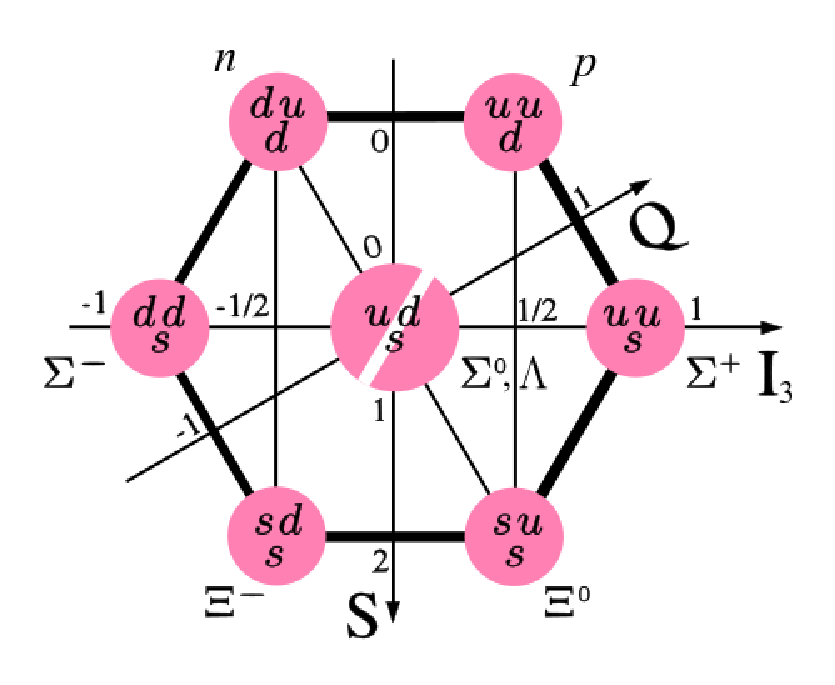
\includegraphics[scale=0.5]{isospin1.eps}
\caption{Baryons with spin $\nicefrac{1}{2}$ or $-\nicefrac{1}{2}$.}\label{fig:isospin1}
\end{center}\end{figure}

\begin{figure}\begin{center}
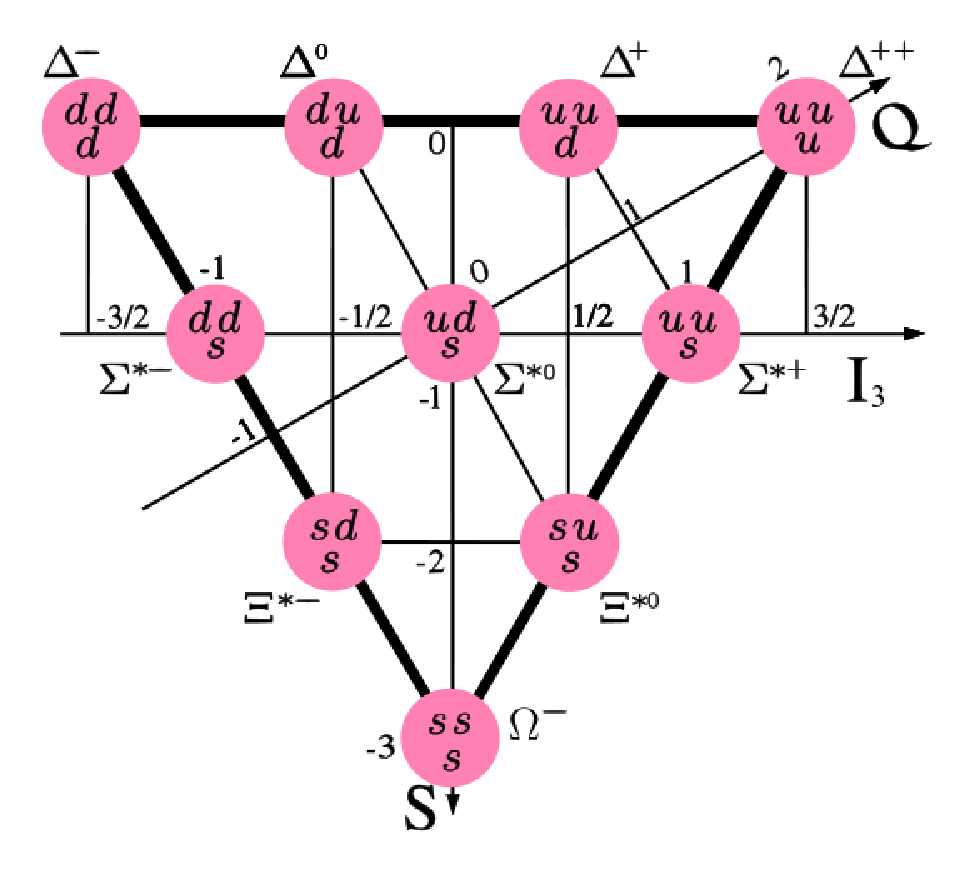
\includegraphics[scale=0.5]{isospin2.eps}
\caption{Baryons with spin $\nicefrac{3}{2}$ or $-\nicefrac{3}{2}$.}\label{fig:isospin2}
\end{center}\end{figure}


\end{document}

